\section{Quasi-Physical Simulation for UV motion control}


\begin{frame}{Quasi-Physical Simulation for UV motion control}
	\framesubtitle{Mathworks AUV}
	\begin{tikzpicture}[remember picture,overlay]
		% \node[fill=blue!30, text=white, font=\large, rounded corners] 
		\node at (current page.north east) [xshift=-6.5cm, yshift=-3cm] 
		{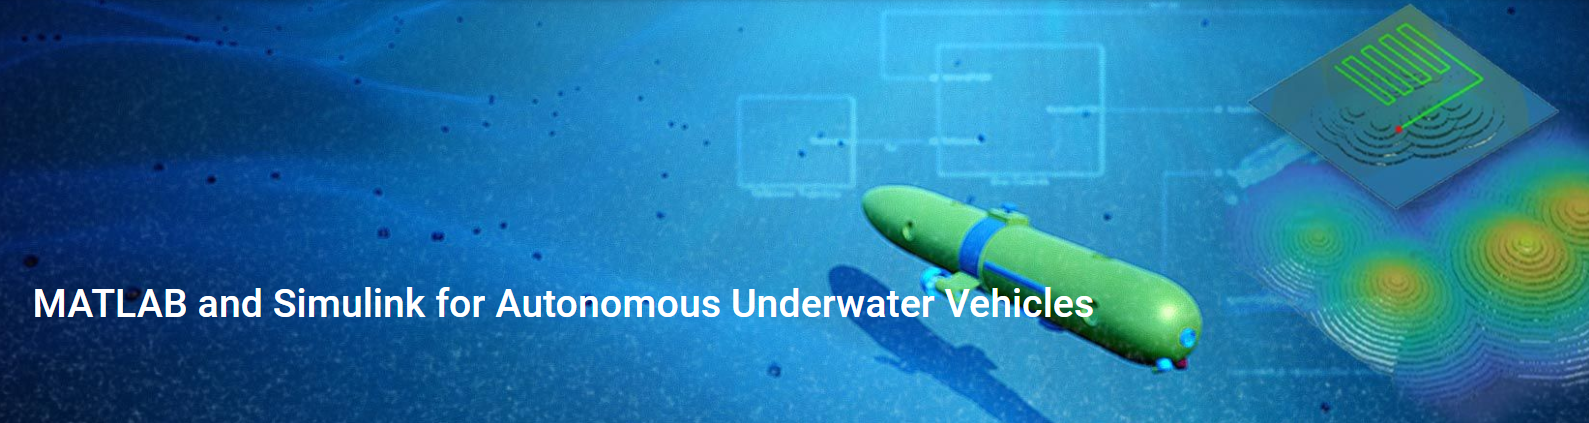
\includegraphics[width=\linewidth]{img/simscape_UUV.png}};
	\end{tikzpicture} 
	
	\begin{tikzpicture}[remember picture,overlay]
		% \node[fill=blue!30, text=white, font=\large, rounded corners] 
		\node at (current page.north east) [xshift=-3cm, yshift=-7cm] 
		{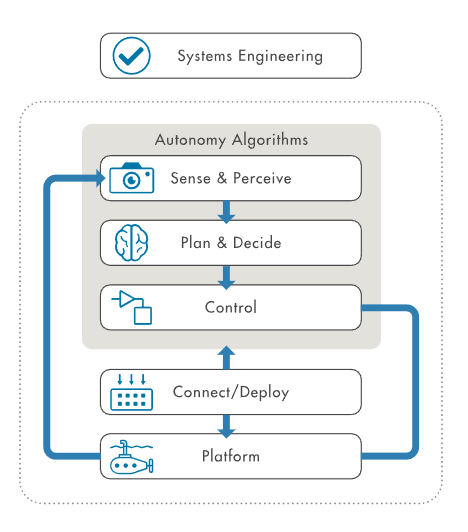
\includegraphics[width=0.35\linewidth]{img/simscape_UUV1.png}};
	\end{tikzpicture} 
	
	
	\vspace{2.5cm}
	\begin{columns}[onlytextwidth]
		\column{.5\textwidth}
		Interdisciplinary teams can use MATLAB and Simulink as a common integration environment throughout the entire autonomous underwater vehicle workflow. From systems engineering to platform modeling, environment simulation, and autonomy algorithm design, Model-Based Design helps you reduce risk and build confidence in system performance well in advance of the sea trial.\column{.5\textwidth}
	\end{columns}
\end{frame}


% =========================================
% =========================================




\begin{frame}{Quasi-Physical Simulation for UV motion control}
	\framesubtitle{Mathworks AUV}
	\begin{tikzpicture}[remember picture,overlay]
		% \node[fill=blue!30, text=white, font=\large, rounded corners] 
		\node at (current page.north east) [xshift=-6.25cm, yshift=-4cm] 
		{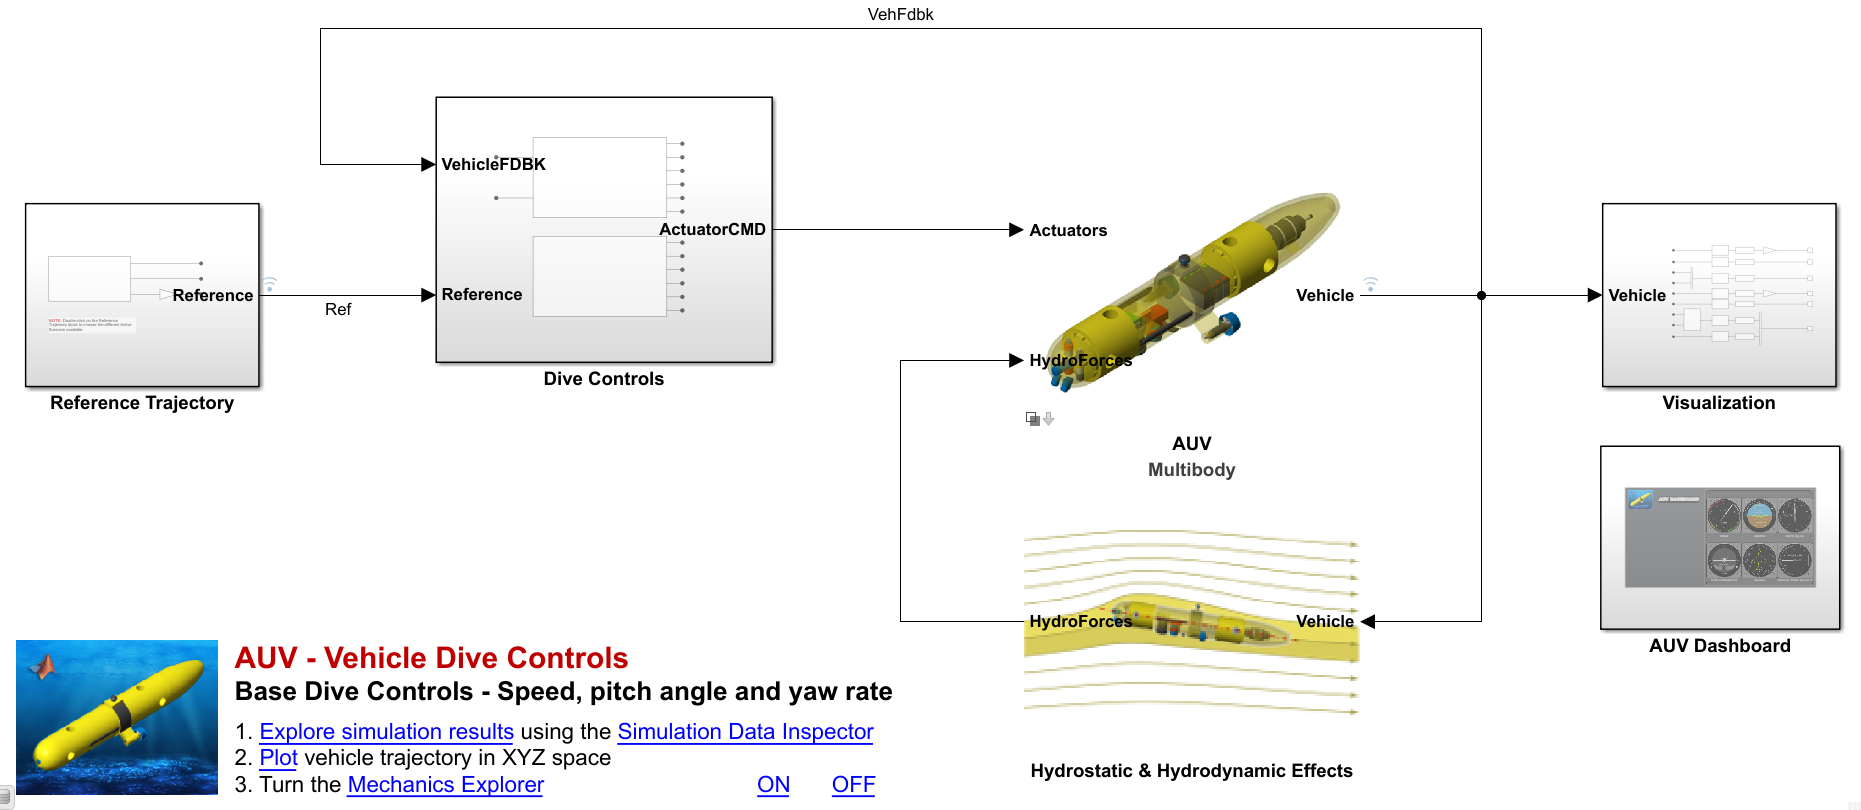
\includegraphics[width=\linewidth]{img/Simulation.png}};
	\end{tikzpicture} 
	\vspace{5cm}
	
	Simspace Multibody is used to simulate the mathimatical model of the vehicle.
	
	Simspace Multibody ultilizes a combination of interconnected bodies (inertias), joints and constrants (relative DoFs) and force elements to solve the dynamics of the model
\end{frame}


% =========================================
% =========================================


\begin{frame}{Quasi-Physical Simulation for UV motion control}
	\framesubtitle{Mathworks AUV}
	\begin{tikzpicture}[remember picture,overlay]
		% \node[fill=blue!30, text=white, font=\large, rounded corners] 
		\node at (current page.north east) [xshift=-6.5cm, yshift=-5cm] 
		{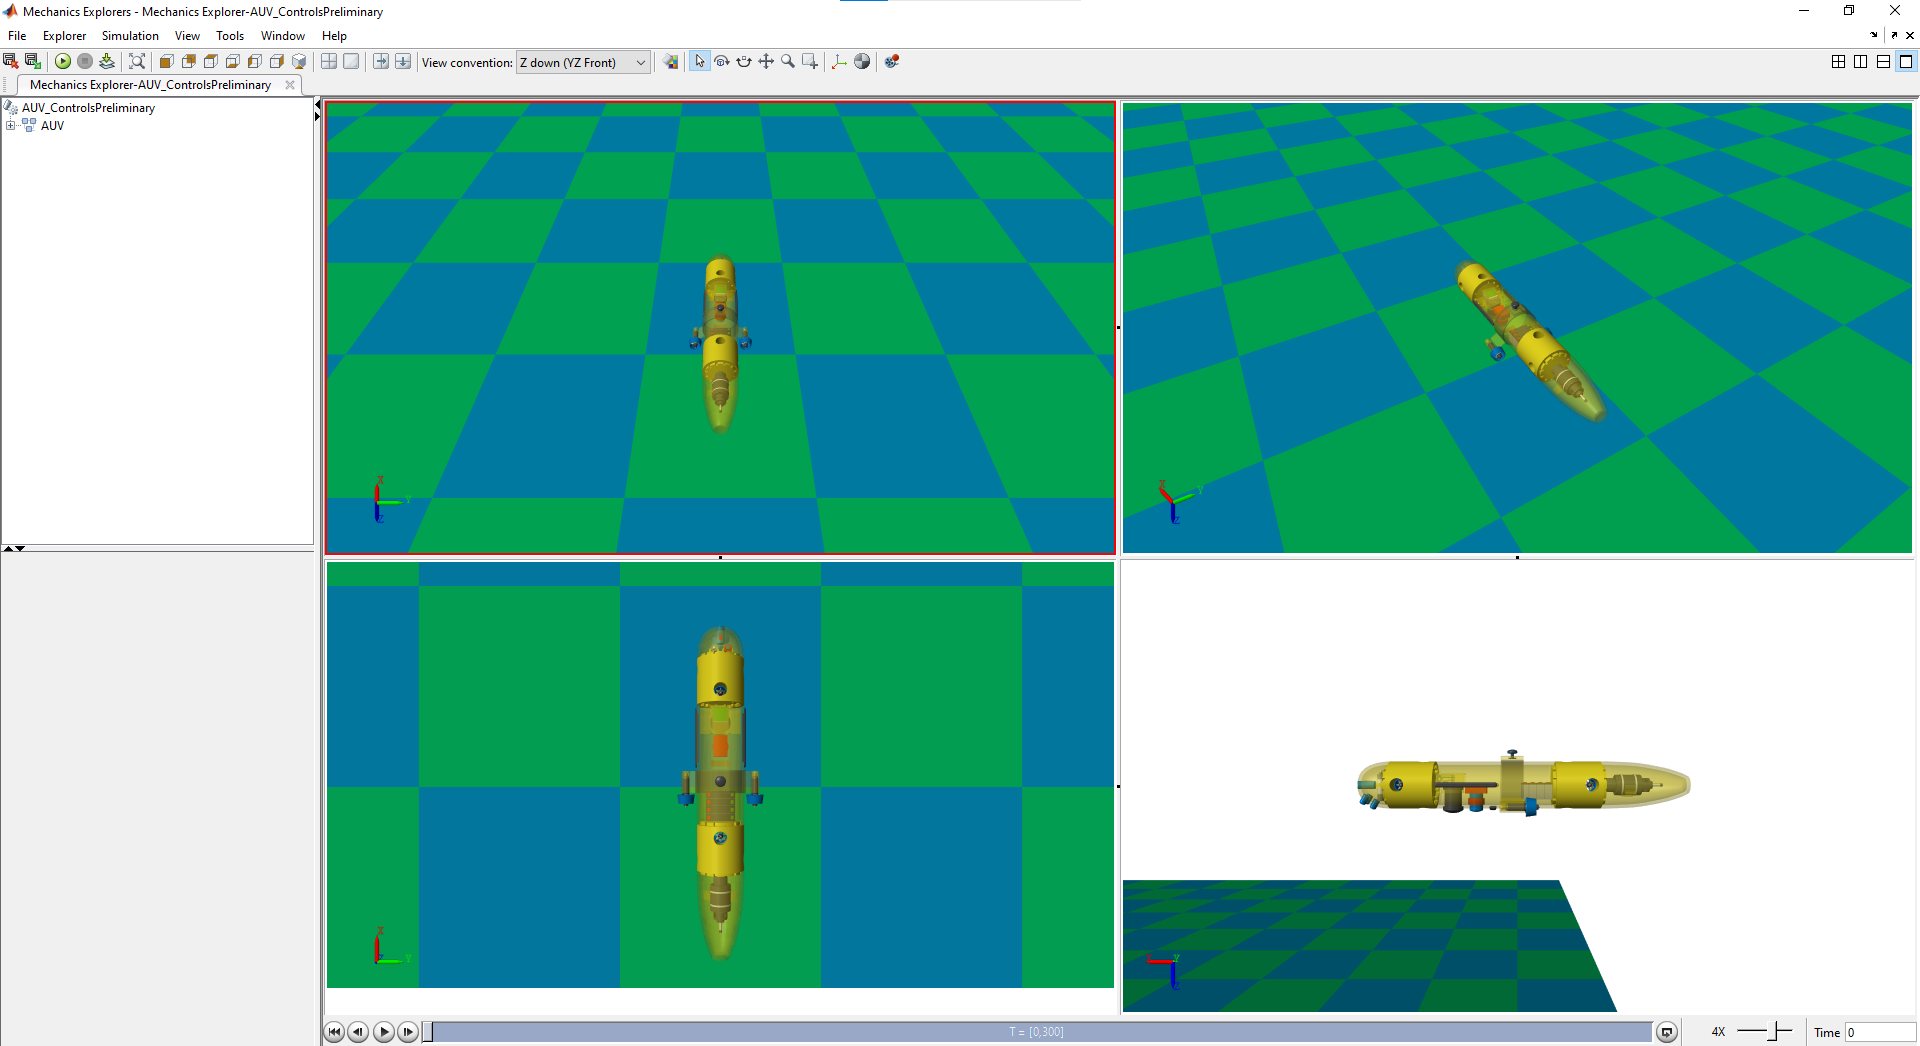
\includegraphics[width=\linewidth]{img/AUV_simscape 1.png}};
	\end{tikzpicture} 
\end{frame}


% =========================================
% =========================================

\begin{frame}{Quasi-Physical Simulation for UV motion control}
	\framesubtitle{Mathworks AUV}
	\begin{tikzpicture}[remember picture,overlay]
		% \node[fill=blue!30, text=white, font=\large, rounded corners] 
		\node at (current page.north east) [xshift=-1.5cm, yshift=-4.7cm] 
		{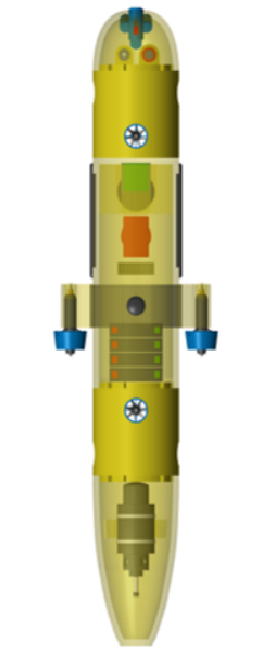
\includegraphics[width=0.17\linewidth]{img/Model.png}};
	\end{tikzpicture} 
	
	IMU located in the main
	hum, 6 actuators:
	\begin{itemize}
		\item BowVerThurster (vertical thurster located at the front of AUV)
		\item BowHorThurster (horizontal thurster located at the front of AUV)
		\item StarboardProp (Right Propeller) 
		\item PortProp (Left Propeller)
		\item SternVerThurster (vertical thurster located at the back of AUV)
		\item SternHorThurster (horizontal thurster located at the back of AUV)
	\end{itemize}
\end{frame}





% =========================================
% =========================================




\begin{frame}{Quasi-Physical Simulation for UV motion control}
	\framesubtitle{Mathworks AUV}
	\begin{tikzpicture}[remember picture,overlay]
		% \node[fill=blue!30, text=white, font=\large, rounded corners] 
		\node at (current page.north east) [xshift=-6.25cm, yshift=-4cm] 
		{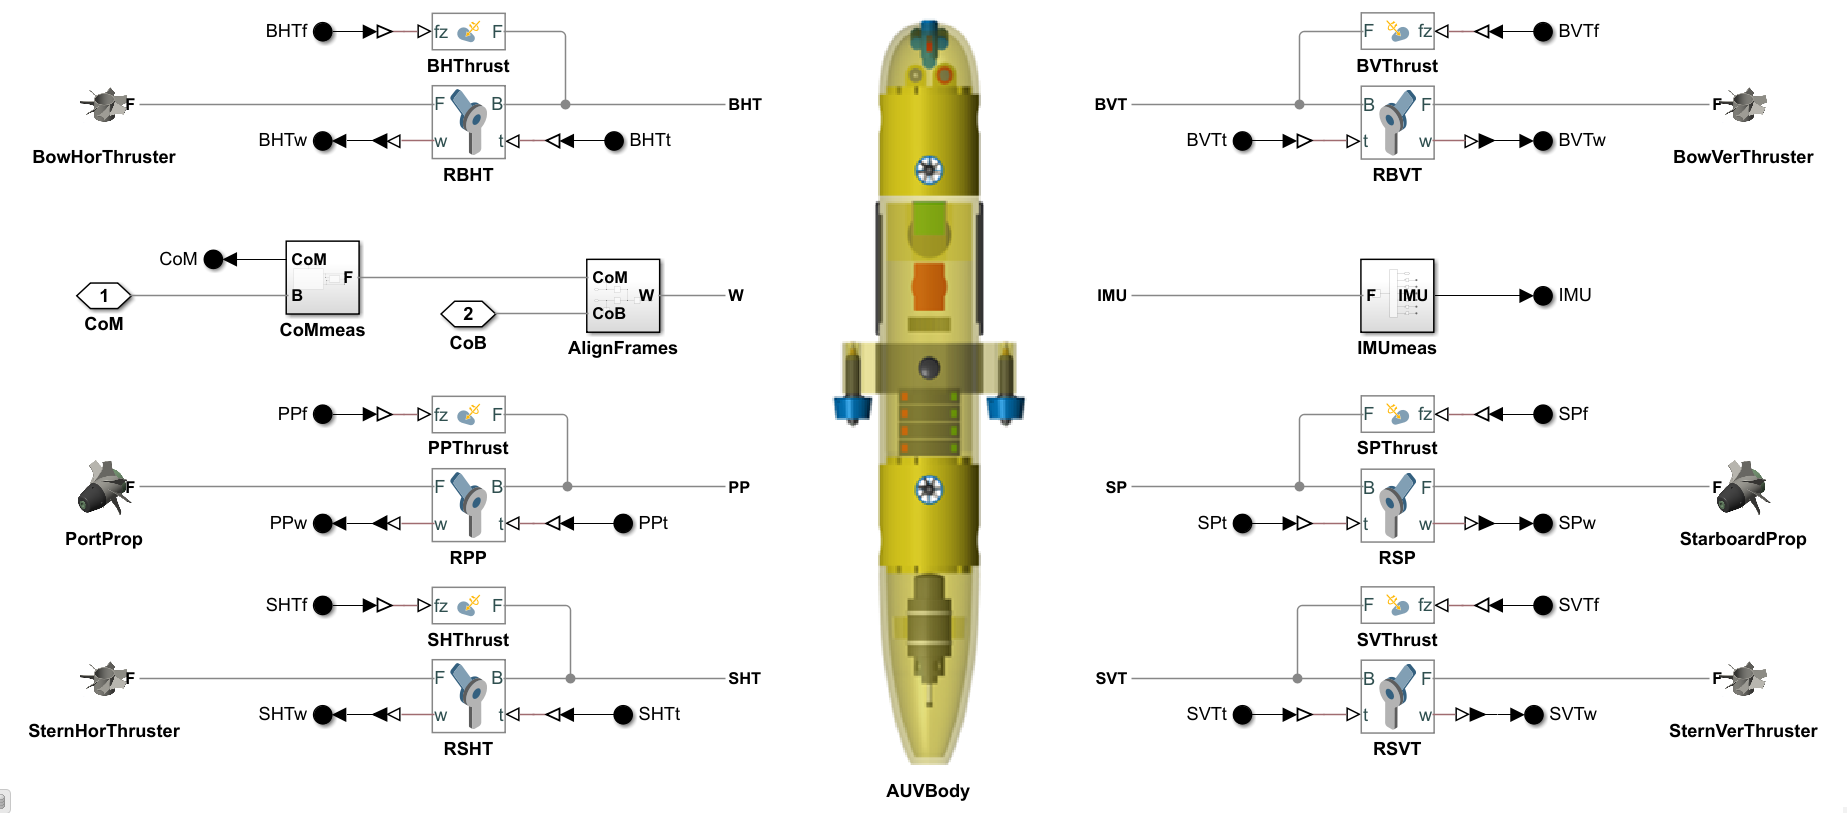
\includegraphics[width=\linewidth]{img/AUV_simscape.png}};
	\end{tikzpicture} 
	\vspace{5cm}
	
	To describe the behavior of a multi-body system, we define the corresponding coordinates and attached forces
\end{frame}



% =========================================
% =========================================

\begin{frame}{Quasi-Physical Simulation for UV motion control}
	\framesubtitle{Mathworks AUV}
	\begin{tikzpicture}[remember picture,overlay]
		% \node[fill=blue!30, text=white, font=\large, rounded corners] 
		\node at (current page.north east) [xshift=-3cm, yshift=-3cm] 
		{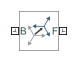
\includegraphics[width=0.15\linewidth]{img/rigid_transform.png}};
	\end{tikzpicture} 
	
	\begin{tikzpicture}[remember picture,overlay]
		% \node[fill=blue!30, text=white, font=\large, rounded corners] 
		\node at (current page.north east) [xshift=-3cm, yshift=-5cm] 
		{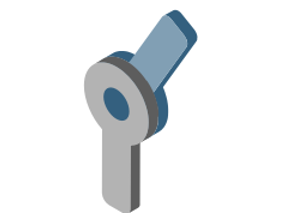
\includegraphics[width=0.15\linewidth]{img/AUVRevoluteJoint.png}};
	\end{tikzpicture} 
	
	\begin{tikzpicture}[remember picture,overlay]
		% \node[fill=blue!30, text=white, font=\large, rounded corners] 
		\node at (current page.north east) [xshift=-3cm, yshift=-7cm] 
		{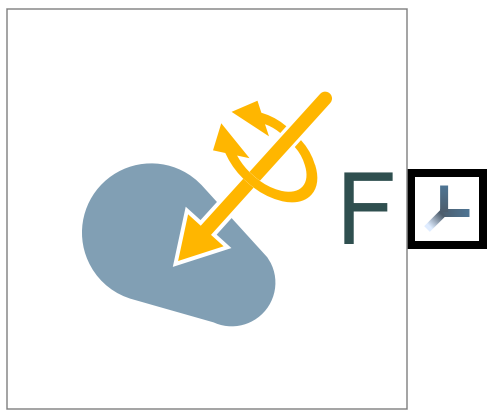
\includegraphics[width=0.09\linewidth]{img/TheExternalForceandTorque.png}};
	\end{tikzpicture}
	
	\vspace{-1.5cm}
	\begin{itemize}
		\item Body frames can be created using body elements block with preset shapes and connected using \textcolor{blue}{rigid transform blocks}
		
		\vspace{1cm}
		\item \textcolor{blue}{Joint blocks} connect the frames and impose kinetic constraints and determine how they move relative to each other
		
		\vspace{1cm}
		\item \textcolor{blue}{The External Force and Torque} represents forces or torques applied on the multibody model.
		
		\vspace{1cm}
		\item \textcolor{blue}{File Solid Block} assosiates individual part files from CAD formats to body blocks in the model.
	\end{itemize}
\end{frame}

% =========================================
% =========================================

\begin{frame}{Quasi-Physical Simulation for UV motion control}
	\framesubtitle{Mathworks AUV}
	\begin{tikzpicture}[remember picture,overlay]
		% \node[fill=blue!30, text=white, font=\large, rounded corners] 
		\node at (current page.north east) [xshift=-4cm, yshift=-5cm] 
		{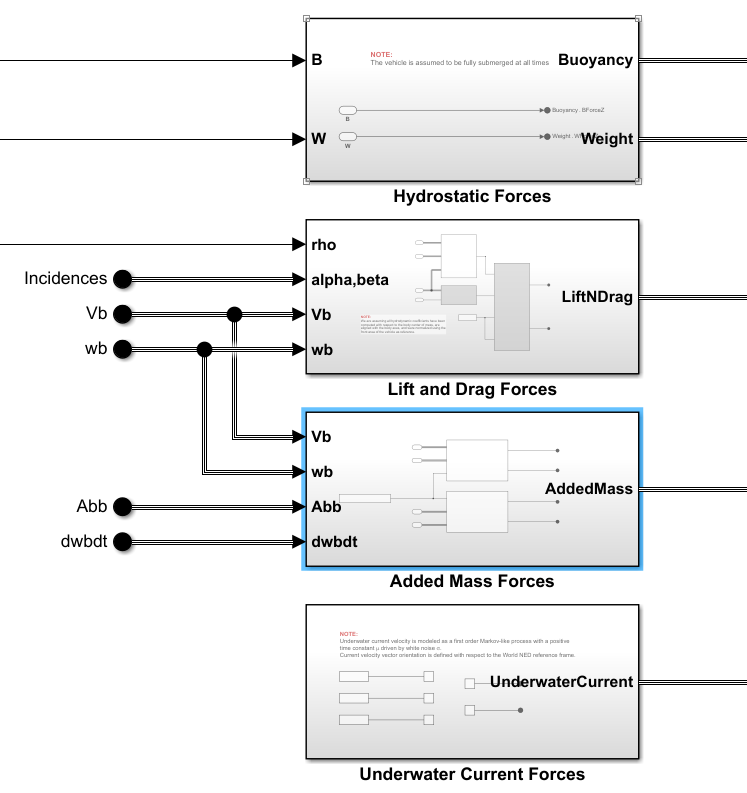
\includegraphics[width=0.5\linewidth]{img/HydrostaticandHydrodynamics.png}};
	\end{tikzpicture}
	
	\vspace{3cm}
	Represents external forces of 
	
	the marine environment. 
	
	Forces consist of:
	\begin{itemize}
		\item Gravity and buoyancy effects
		\item Lift and drag forces
		\item Added mass effects
		\item Underwater current forces
	\end{itemize}
\end{frame}

% =========================================
% =========================================


\begin{frame}{Quasi-Physical Simulation for UV motion control}
	\framesubtitle{Mathworks AUV}
	
	
	
	\begin{tikzpicture}[remember picture,overlay]
		% \node[fill=blue!30, text=white, font=\large, rounded corners] 
		\node at (current page.north east) [xshift=-6cm, yshift=-3.2cm] 
		{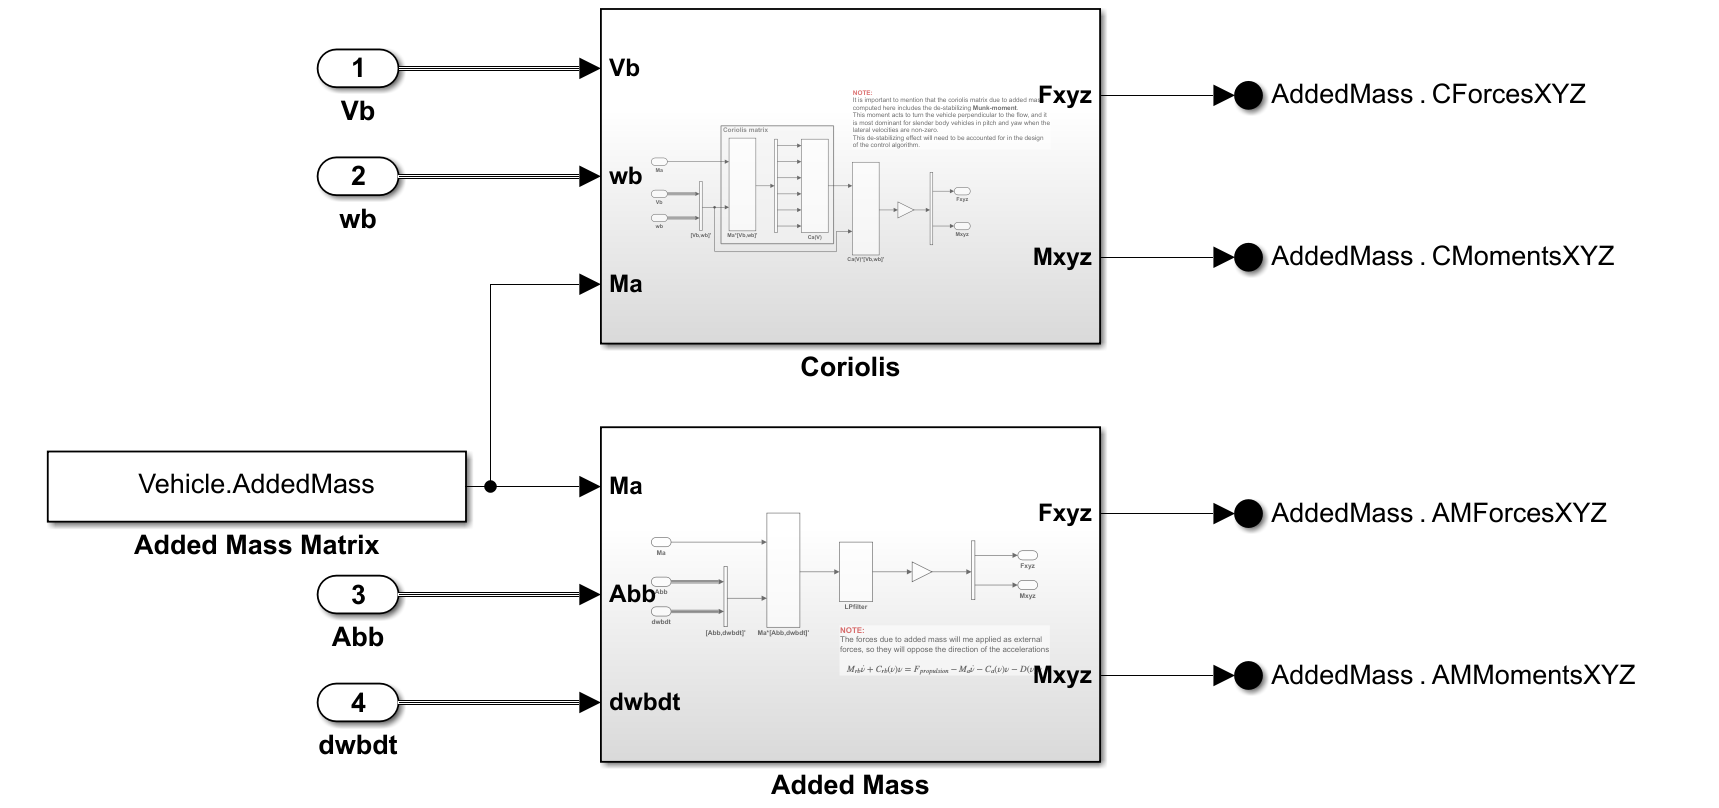
\includegraphics[width=0.65\linewidth]{img/AddedMassandCoriolis.png}};
	\end{tikzpicture}
	
	\vspace{2.5cm}
	
	\begin{block}{Mathematical model}
		\begin{align}
			(M_{RB} + M_A) \dot{\nu} + (C_{RB}+C_A)(\nu) \nu + 
			D(\nu_r) \nu_r
			+\underbrace{{g(\eta) + g_o}}_{\text{hydrostatic forces}}
			= F_{propulsion}
		\end{align}
		
		where $M_A$ is the added mass matrix and $C_A$ is the coriolis effect induced by the added mass 
	\end{block}
	
	
\end{frame}

% =========================================
% =========================================


\begin{frame}{Quasi-Physical Simulation for UV motion control}
	\framesubtitle{Mathworks AUV}
	
	\begin{columns}[onlytextwidth]
		\column{.5\textwidth}
		\begin{block}{Added mass}
			The elongated myring shape of the hull results in \begin{align*}
				M_A =\begin{bmatrix}
					m_{11} & 0 & 0 & 0 & 0 & 0 \\
					0 & m_{22} & 0 & 0 & 0 & m_{26} \\
					0 & 0 & m_{33} & 0 & m_{35} & 0 \\
					0 & 0 & 0 & 0 & 0 & 0 \\
					0 & 0 & m_{53} & 0 & m_{55} & 0 \\
					0 & m_{62} & 0 & 0 & 0 & m_{66}
				\end{bmatrix}        
			\end{align*}
			\begin{align*}
				m_{22} = m_{53} \hspace{0.2cm} and \hspace{0.2cm} m_{55} = m_{66}
			\end{align*}
		\end{block}
		\column{.5\textwidth}
	\end{columns}
	
	\begin{tikzpicture}[remember picture,overlay]
		% \node[fill=blue!30, text=white, font=\large, rounded corners] 
		\node at (current page.north east) [xshift=-3.5cm, yshift=-3cm] 
		{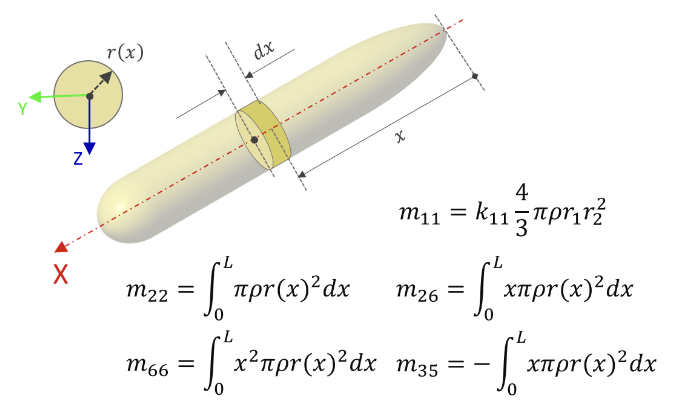
\includegraphics[width=0.4\linewidth]{img/Addedmasscalc.png}};
	\end{tikzpicture}
	
	\begin{tikzpicture}[remember picture,overlay]
		% \node[fill=blue!30, text=white, font=\large, rounded corners] 
		\node at (current page.north east) [xshift=-3.5cm, yshift=-7cm] 
		{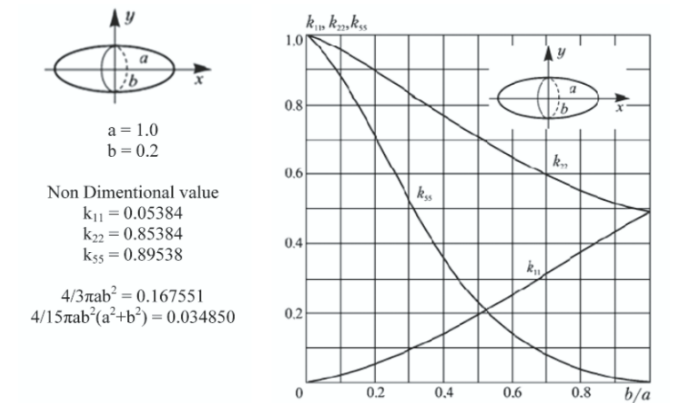
\includegraphics[width=0.4\linewidth]{img/AlsoAddedmasscalc.png}};
	\end{tikzpicture}
	
	
	
\end{frame}

% =========================================
% =========================================

\begin{frame}{Quasi-Physical Simulation for UV motion control}
	\framesubtitle{Mathworks AUV}
	\begin{tikzpicture}[remember picture,overlay]
		% \node[fill=blue!30, text=white, font=\large, rounded corners] 
		\node at (current page.north east) [xshift=-3.5cm, yshift=-3.5cm] 
		{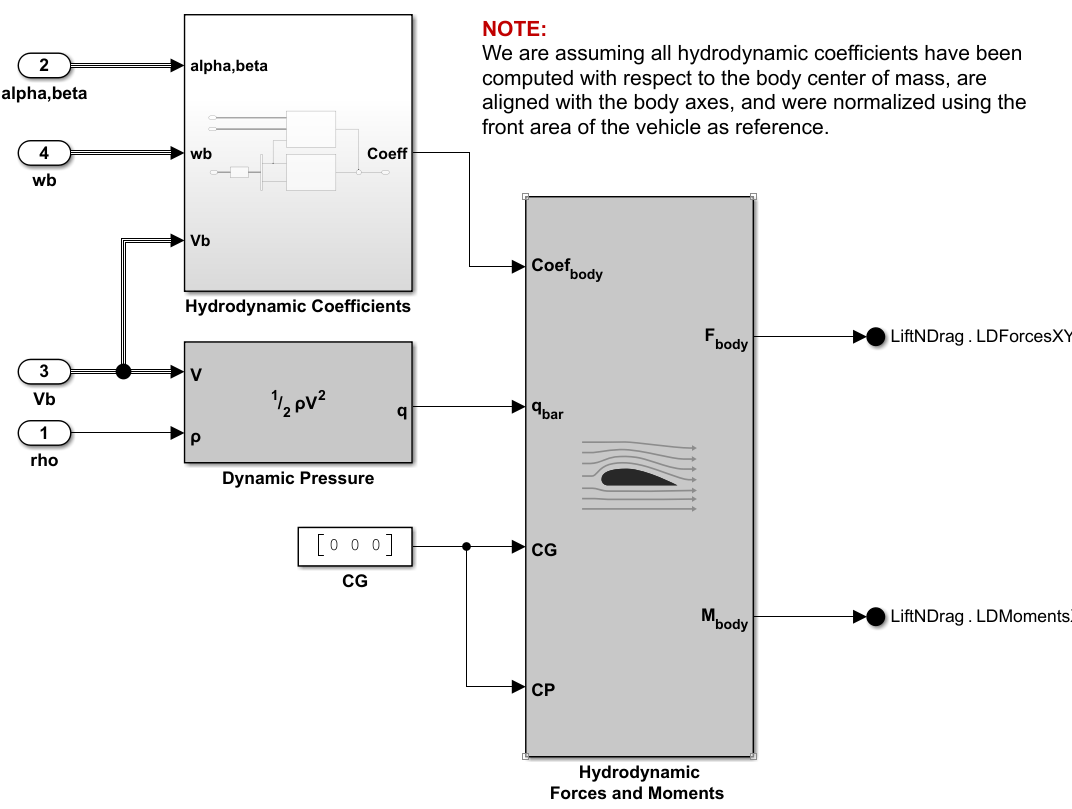
\includegraphics[width=0.5\linewidth]{img/LiftandDrag.png}};
	\end{tikzpicture}
	
	\begin{tikzpicture}[remember picture,overlay]
		% \node[fill=blue!30, text=white, font=\large, rounded corners] 
		\node at (current page.north east) [xshift=-3.5cm, yshift=-7.5cm] 
		{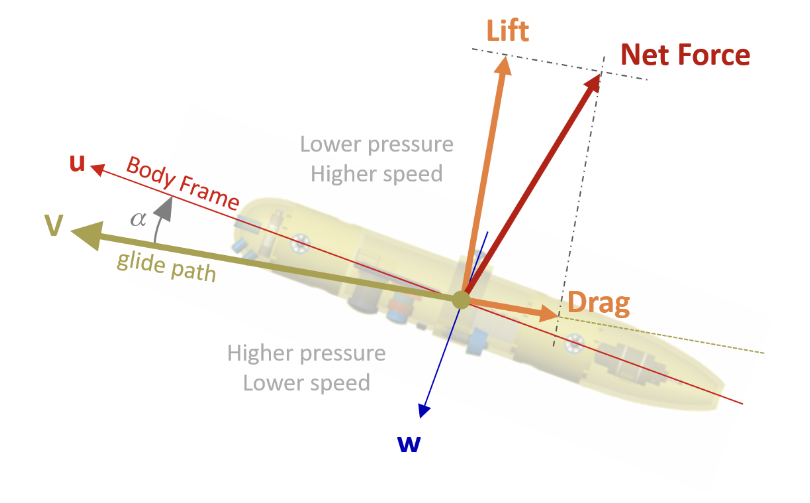
\includegraphics[width=0.4\linewidth]{img/DragNLiftillustration.png}};
	\end{tikzpicture}
	
	\vspace{-1cm}
	\begin{columns}[onlytextwidth]
		\column{.45\textwidth}
		\begin{block}{Drag and lift forces}
			\begin{align*}
				F_{drag} = \frac{1}{2}\rho V^2 C_d A\\
				F_{lift} = \frac{1}{2}\rho V^2 C_l A
			\end{align*}
			
			where $C_d$ and $C_l$ are normally from experiments and used in practice
		\end{block}
		\column{.5\textwidth}
	\end{columns}
\end{frame}

% =========================================
% =========================================

\begin{frame}{Quasi-Physical Simulation for UV motion control}
	\framesubtitle{Mathworks AUV}
	\begin{tikzpicture}[remember picture,overlay]
		% \node[fill=blue!30, text=white, font=\large, rounded corners] 
		\node at (current page.north east) [xshift=-5cm, yshift=-5cm] 
		{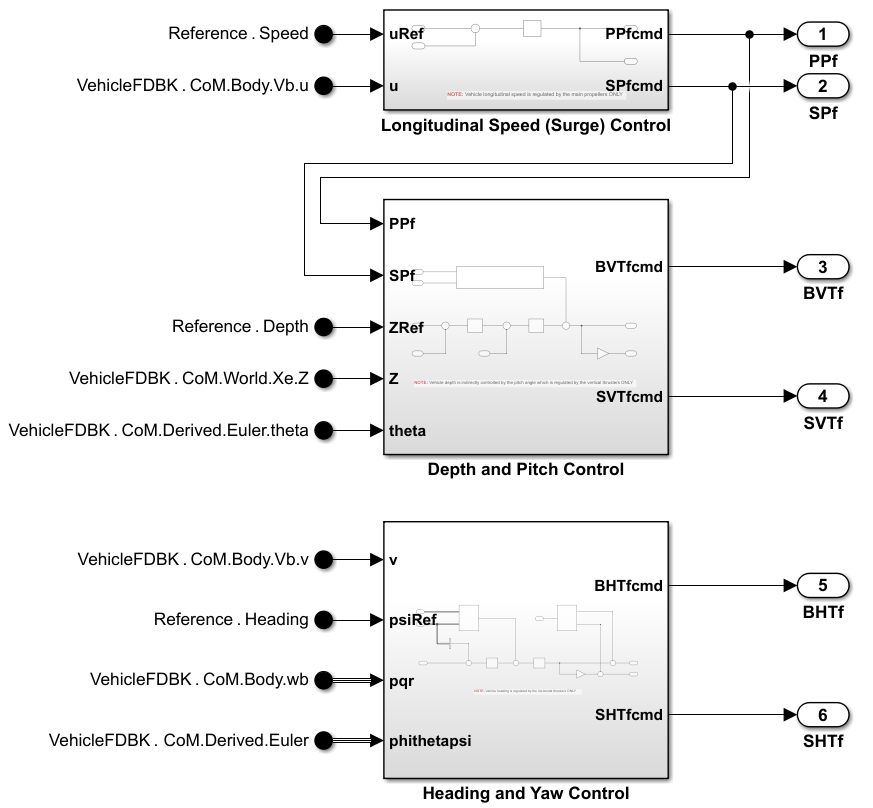
\includegraphics[width=0.6\linewidth]{img/Controller.png}};
	\end{tikzpicture}
	
	
	\vspace{5cm}
	3 Controllers
	\begin{itemize}
		\item Surge Controller
		\item Heave and Pitch Controller
		\item Yaw Controller
	\end{itemize}
\end{frame}



% =========================================
% =========================================

\begin{frame}{Quasi-Physical Simulation for UV motion control}
	\framesubtitle{Mathworks AUV}
	\begin{tikzpicture}[remember picture,overlay]
		% \node[fill=blue!30, text=white, font=\large, rounded corners] 
		\node at (current page.north east) [xshift=-8cm, yshift=-3cm] 
		{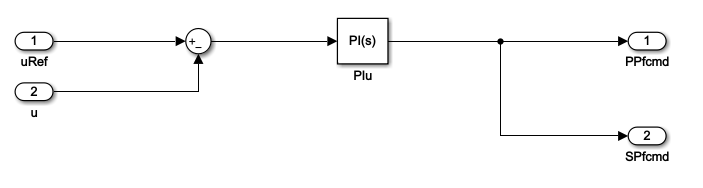
\includegraphics[width=0.4\linewidth]{img/SurgeController.png}};
	\end{tikzpicture}
	
	\begin{tikzpicture}[remember picture,overlay]
		% \node[fill=blue!30, text=white, font=\large, rounded corners] 
		\node at (current page.north east) [xshift=-8cm, yshift=-5.5cm] 
		{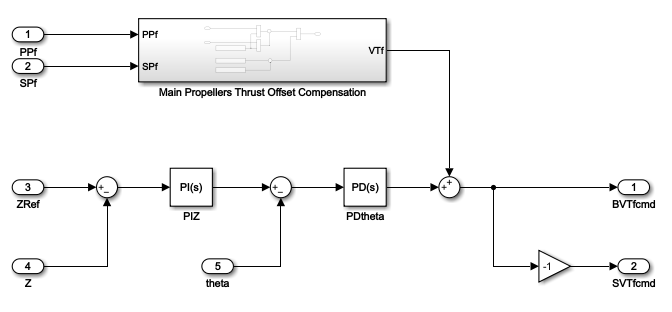
\includegraphics[width=0.4\linewidth]{img/HeaveandPitchController.png}};
	\end{tikzpicture}
	
	\begin{tikzpicture}[remember picture,overlay]
		% \node[fill=blue!30, text=white, font=\large, rounded corners] 
		\node at (current page.north east) [xshift=-8cm, yshift=-8cm] 
		{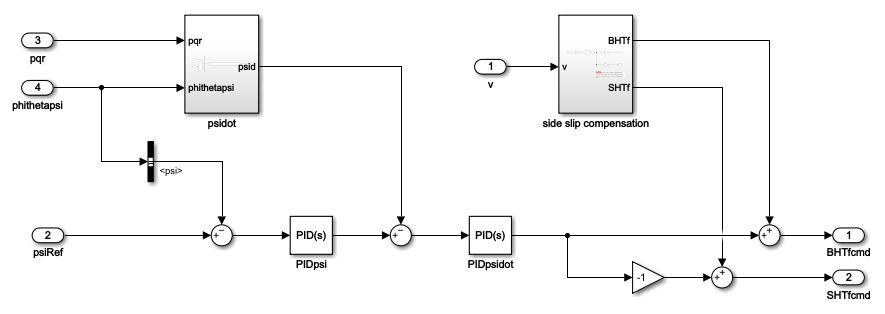
\includegraphics[width=0.4\linewidth]{img/YawController.png}};
	\end{tikzpicture}
	
	\vspace{-1cm}
	\begin{itemize}
		\item Surge Controller controls both propellers
		
		\vspace{1.5cm}
		\item Heave and Pitch Controller controls vertical thursters
		
		\vspace{2.5cm}
		
		
		\item Yaw Controller controls horizontal thursters
	\end{itemize}
	
	\vspace{5.5cm}
\end{frame}




% =========================================
% =========================================




